\documentclass[11pt]{article}

\usepackage[letterpaper]{geometry}

\usepackage[utf8]{inputenc}
\usepackage{mathpazo}
\usepackage{amsmath}
\usepackage{amsfonts}
\usepackage{physics}
\usepackage{siunitx}

\usepackage{fancyhdr}

\usepackage{graphicx}
\usepackage{float}
\usepackage{booktabs}

\usepackage[shortlabels,inline]{enumitem}

% Hyperlinks with decent looking default colors.
\usepackage{hyperref}
\usepackage{xcolor}
\hypersetup{
  colorlinks,
  linkcolor={red!50!black},
  citecolor={blue!50!black},
  urlcolor={blue!80!black}
}

% For those sexy spaced low small caps from classic-thesis!
\usepackage{microtype}
\usepackage{textcase}
\DeclareRobustCommand{\spacedlowsmallcaps}[1]{%
  \textls[80]{\scshape\MakeTextLowercase{#1}}%
}

\pagestyle{fancy} 
\fancyhead{}
\rhead{Ali Ramadhan}
\lhead{12.818: Project one}
\chead{}
\cfoot{\thepage}

\title{\spacedlowsmallcaps{\small 12.818: Introduction to Atmospheric Data and Large-scale Dynamics}\\ \spacedlowsmallcaps{\Large Project two: Hydrostatic balance and the large-scale tilt of constant pressure surfaces}}
\author{Ali Ramadhan}
\date{\today}

% \renewcommand\thesection{\Alph{section}}

\begin{document}
\maketitle

In this project we will use the concept of hydrostatic balance to estimate the \emph{tilt} of isobaric pressure surfaces in the atmosphere from the poles to the equator. The monthly/seasonal composite plots in this project were produced using NCEP\footnotemark~reanalysis data averaged from Janurary 1948 to August 2017.  The Earth System Research Laboratory of the Physical Sciences Division of NOAA provides a convenient \href{ https://www.esrl.noaa.gov/psd/cgi-bin/data/composites/printpage.pl}{web page} for producing these plots.

\footnotetext{The United States National Centers for Environmental Prediction (NCEP) is a collection of nine centers and is a child agency of the National Weather Service, which is itself a child agency of the National Oceanic and Atmospheric Administration (NOAA).}

\section{Maps}
Figure \ref{fig:GeoHeight500hPa} shows a hemispheric map of the geopotential height at \SI{500}{\hecto\Pa} for the month of January. We note that the geopotential height is lower at the North Pole, and progressively increases with longitude towards the the equator. The geopotential height is not radially symmetric due to the presence of land masses and thus varies slightly as a function of latitude. Between \SIrange{20}{60}{\degree N} along North America (the black line from the North Pole downwards in figure \ref{fig:GeoHeight500hPa}), say from Hudson's Bay to the Gulf of Mexico, we see that the geopotential height increased by about \SI{700}{\m} from \SI{5100}{\m} to \SI{5800}{\m}.

\begin{figure}
	\centering
	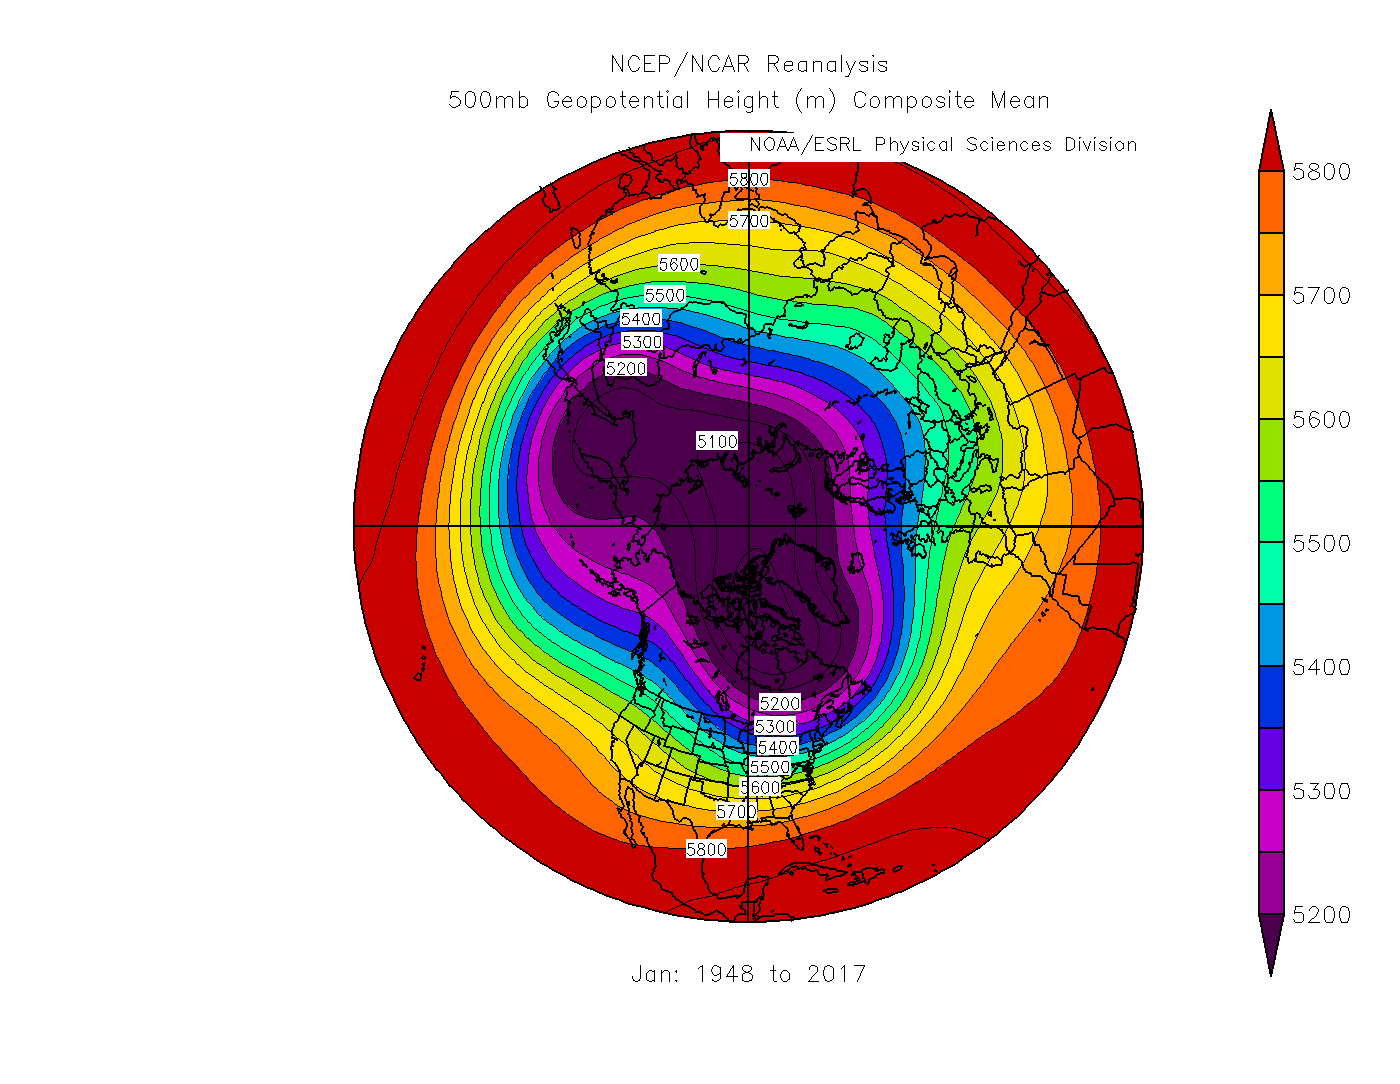
\includegraphics[width=\textwidth]{GeoHeight500hPa.png}
	\caption{The geopotential height of the \SI{500}{\hecto\Pa} constant pressure surface in meters (m) over the northern hemisphere in January. This plot was produced using NCEP reanalysis data averaged over the years 1948--2017.}
	\label{fig:GeoHeight500hPa}
\end{figure}

Figure \ref{fig:AirT700hPa} shows a hemispheric map of the air temperature at \SI{700}{\hecto\Pa} for the month of January. Looking at the difference in air temperature from \SIrange{20}{60}{\degree N} along North America again, we note an increase in temperature by about \SI{30}{\degreeCelsius}, from \SI{-25}{\degreeCelsius} in Hudson's Bay to \SI{5}{\degreeCelsius} in the Gulf of Mexico.

\begin{figure}
  \centering
  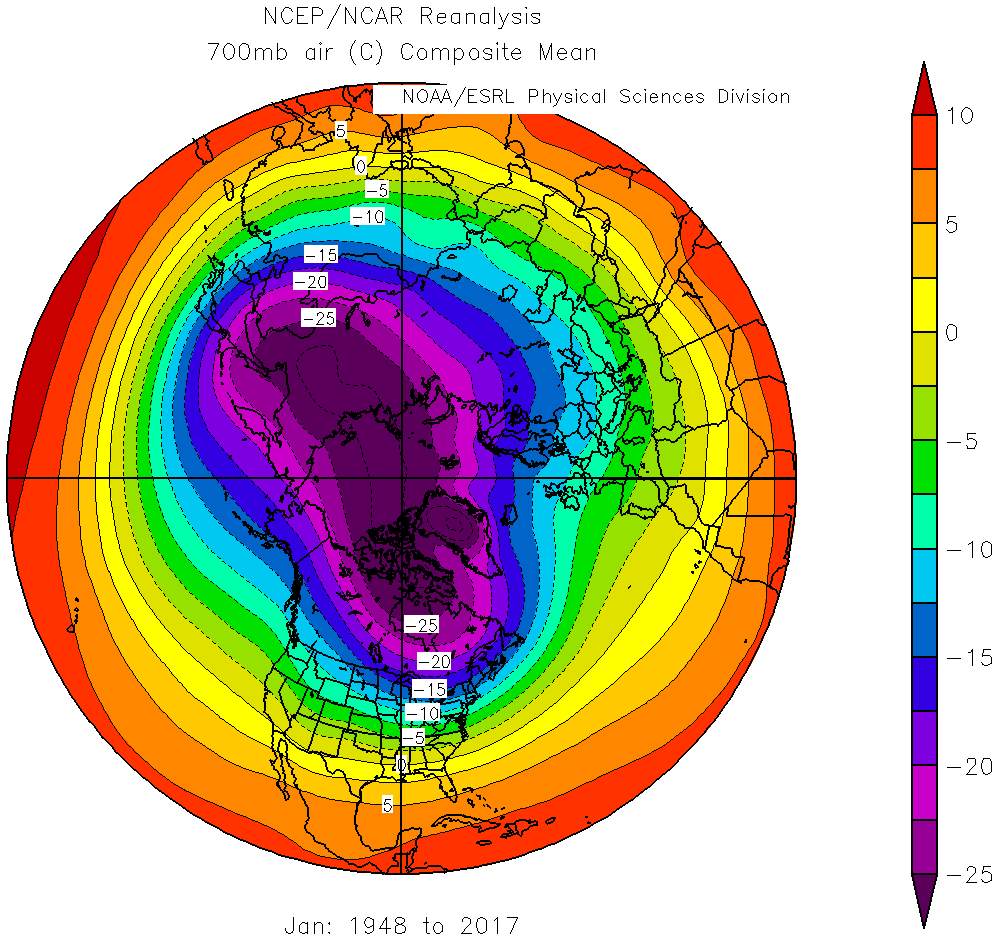
\includegraphics[width=\textwidth]{AirT700hPa.png}
  \caption{The air temperature at the \SI{700}{\hecto\Pa} constant pressure surface in degrees Celcius (\SI{}{\degreeCelsius}) over the northern hemisphere in January. This plot was produced using NCEP reanalysis data averaged over the years 1948--2017.}
  \label{fig:AirT700hPa}
\end{figure}

\section{Hydrostatic balance and the tilt of a constant pressure surface}
The atmosphere is largely just a fluid or gas obeying the ideal gas law
\begin{equation} \label{eq:IGL}
  p = \rho RT
\end{equation}
where $p$ is the pressure of the ideal gas, $\rho$ is its density, $T$ is its temperature, and $R = \SI{8.31445}{\J/\mol.\K}$ is the universal gas constant. When considering a specific gas or mixture of gases, the gas constant must be replaced by a specific gas constant $R_s = R/M$ where $M$ is the molar mass of the specific gas. In the case of Earth's atmosphere, we will take this specific gas to be dry air\footnotetext{In the case of moist air, which is a mixture of dry air and water vapor, the percentage of water vapor is taken into account by keeping the specific gas constant for dry air while using the \emph{virtual temperature} $$ T_v = \frac{T\left( 1 + r_v/\epsilon \right)}{1+r_v} $$ in place of the temperature. Here $\epsilon \approx 0.622$ if the ratio of the specific gas constants for dry air and water vapor and $r_v$ is the mixing ratio of water vapor mass to dry air mass. Physically, the virtual temperature is the temperature that dry air would have if its pressure and density were equal to those of the moist air. It essentially allows us to apply the equation of state for dry air to moist air \cite{AMSVirtualTemp}.}, which consists mainly of nitrogen (78\% by volume) and oxygen (21\% by volume) along with various other trace gases\footnotemark~ leading to a molar mass of $M = \SI{28.97}{\g/\mol}$ and a specific gas constant of $R_s = \SI{287.058}{\J/\kg.\K}$. Note the change of units from the universal to the specific gas constant.

\footnotetext{Argon, carbon dioxide, neon, helium, and methane in order of decreasing concentration as well as water vapor which strongly varies locally \cite{Wallace}.}

The variation of the Earth's atmosphere's pressure with height is governed by the concept of \emph{hydrostatic balance}. Gravity alone, in the absence of the pressure force, would cause the Earth's atmosphere to collapse to a thin\footnotemark~shell entirely located at the surface. And the pressure force alone, in the absence of gravity, would cause the Earth's atmosphere to diffuse to outer space. However, in the presence of each other the two forces balance each other out to create an atmosphere that forms a shell around the Earth concentrated near the surface. Mathematically, this balance represents a steady-state solution of the Navier-Stokes equations and can be written as
\begin{equation} \label{eq:HB}
  \frac{\partial p}{\partial z} + \rho g = 0
\end{equation}
where $z$ is the height coordinate and we will let $g \equiv g_0 = \SI{9.80665}{\m/\s^2}$ be defined by the standard acceleration due to gravity.

\footnotetext{This could have been an infinitesimally thin shell had it not been for the electromagnetic force.}

Assuming the atmosphere is vertically isothermal and that atmospheric pressure varies with height only, we can use equation \eqref{eq:IGL} to write $\rho = p/R_sT$ and substitute it into \eqref{eq:HB} to obtain
\begin{equation*}
  \frac{dp}{dz} = - \frac{g}{R_sT}p
\end{equation*}
which is a first-order differential equation that can be separated to get
\begin{equation*}
\int \frac{dp}{p} = - \frac{g}{R_sT} \int dz \quad \implies \quad \ln p(z) = - \frac{g}{R_sT}z + C
\end{equation*}
where $C$ is an arbitrary constant. Solving for $p(z)$ leads to the barometric formula
\begin{equation} \label{eq:BF}
  p(z) = p_0 \exp{-\frac{g}{R_sT}z}
\end{equation}
where the arbitrary constant was chosen to be $p_0$, the pressure at the surface, so that $p(0) = p_0$. It models the pressure of an isothermal atmosphere as exponentially decreasing with height and with length scale $H = R_sT/g$ where $T$ can be chosen to be the surface temperature.

We could like to use the barometric formula to estimate the tilt of an isobaric surface. First we will solve \eqref{eq:BF} for the height of the isobaric surface
\begin{equation}
  z = - \frac{R_sT}{g} \ln \left( \frac{p}{p_0} \right).
\end{equation}
We will again assume a vertically isothermal atmosphere but allow for the temperature $T$ to vary in the horizontal direction, which will let us write $z_\mathrm{cold} = -(R_sT_\mathrm{cold}/g)\ln(p/p_0)$ and $z_\mathrm{warm} = -(R_sT_\mathrm{cold}/g)\ln(p/p_0)$. The difference provides us with an expression for the for the difference in height of an isobaric surface between warm and cold latitudes
\begin{equation} \label{eq:Deltaz}
  \Delta z_\mathrm{cold}^\mathrm{warm} = z_\mathrm{warm} - z_\mathrm{cold} = -\frac{R_s \Delta T_\mathrm{cold}^\mathrm{warm}}{g} \ln \left( \frac{p}{p_0} \right)
\end{equation}
where $\Delta T_\mathrm{cold}^\mathrm{warm} = T_\mathrm{warm} - T_\mathrm{cold}$ as well.

We can now use \eqref{eq:Deltaz} to estimate the equator to pole slope of the \SI{500}{\hecto\Pa} isobaric surface, but we will use the observed pole to equator temperature gradient from the \SI{700}{\hecto\Pa} isobaric surface in figure \ref{fig:AirT700hPa}, which we found to be $\Delta T_\mathrm{cold}^\mathrm{warm} = \SI{30}{\degreeCelsius}$. With $p_0 = \SI{1000}{\hecto\Pa}$, this yields a tilt of $\Delta z_\mathrm{cold}^\mathrm{warm} = \SI{610}{\m}$.

We previously found that a tilt of about \SI{700}{\m} so this estimate is not completely in disagreement, however it could be improved. A likely physical explanation for this discrepency is that the temperature gradient changes slightly from \SI{700}{\hecto\Pa} to \SI{500}{\hecto\Pa}, although another more likely explanation is that the contour plots in figures \ref{fig:GeoHeight500hPa} and \ref{fig:AirT700hPa} only provide a resolution of \SI{50}{\m} and \SI{5}{\degreeCelsius} respectively. An increase of \SI{5}{\degreeCelsius} in $\Delta T_\mathrm{cold}^\mathrm{warm}$ is enough to retreive $\Delta z_\mathrm{cold}^\mathrm{warm} = \SI{710}{\m}$ which agrees much more closely. Checking with the air temperature plot at \SI{500}{\hecto\Pa}, we still find a temperature gradient of $\Delta T_\mathrm{cold}^\mathrm{warm} = \SI{30}{\degreeCelsius}$, so more precision or resolution is required. Being very specific with the locations would also help as Husdon's Bay and the Gulf of Mexico are rather large geographical features.

\section{Change of tilt with height}
Repeating the same analysis for different isobaric pressure surfaces, we can produce a table of tilts $z_\mathrm{cold}^\mathrm{warm}$ against geopotential height, shown in table \ref{table:tilts}. The NCEP reanalysis plots referenced to perform the calculations are not included to avoid unnecessarily lengthening this report.

\begin{table}[!h]
  \begin{center}
    \begin{tabular}{cc}
      \toprule
      Geopotential height (\SI{}{\hecto\Pa}) & Tilt $\Delta z_\mathrm{cold}^\mathrm{warm}$ (\SI{}{\m}) \\
      \midrule
      850 & 240 \\
      700 & 375 \\
      500 & 700 \\
      300 & 1000 \\
      250 & 1200  \\
      150 & 1100 \\
      100 & 900 \\
      50  & 700 \\
      \bottomrule
    \end{tabular}
  \end{center}
  \caption{The tilt of isobaric pressure surfaces at various geopotential heights from Hudson's Bay to the Gulf of Mexico during the month of January.}
  \label{table:tilts}
\end{table}

Table \ref{table:tilts} shows that the tilt increases progressively with height in the tropopause but once the stratosphere is reached around \SI{250}{\hecto\Pa}, the tilt begins to progressively decrease. A possible explanation for this is the presence of large land masses, the continents, and their mountain ranges which serve to perturb the large-scale circulation of the lower atmosphere leading to tilts in the isobaric pressure surfaces. However, the stratosphere is far enough away from any land masses or barriers such that it may become much more homogenous than the tropopause, leading to smaller tilts.

\begin{thebibliography}{9}
\bibitem{AMSVirtualTemp}
American Meteorological Society, cited 2012: Virtual temperature. Glossary of Meteorology. [Available online at \url{http://glossary.ametsoc.org/wiki/Virtual_temperature}]

\bibitem{Wallace}
Wallace, John M. and Peter V. Hobbs. \textit{Atmospheric Science; An Introductory Survey}. Elsevier. Second Edition, 2006. Chapter 1.
\end{thebibliography}

\end{document}